% Slide 2
\begin{frame}
\frametitle{Earlier Approaches}
\begin{columns}
\column{0.4\textwidth}
\begin{itemize}
\item{Relatively simple, rely on injecting random data}
\item{Mutative Approach}
\item{Generative Approach}
\end{itemize}
\column{0.6\textwidth}
\begin{figure}
\frame{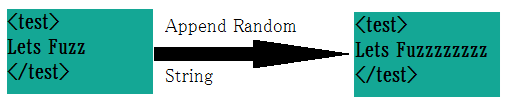
\includegraphics[width=.6\linewidth]{figures/fuzzingStringsMutative.png}}
\caption{Mutative fuzzing of a string.}
\end{figure}
\begin{figure}
\frame{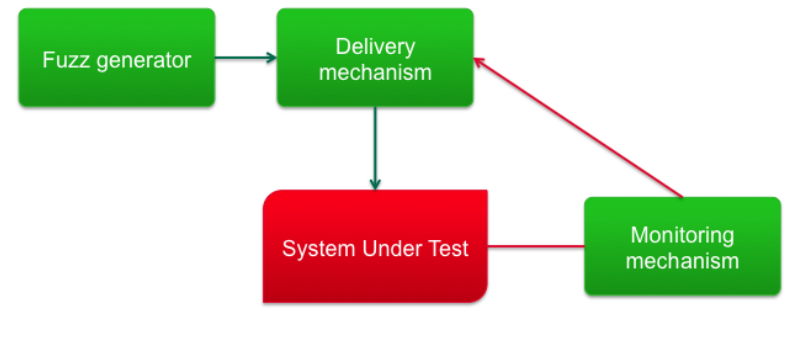
\includegraphics[width=.6\linewidth]{figures/fuzzingAsAConceptGenerative.png}}
\caption{A generative fuzzer creates its own test cases.}
\end{figure}
\end{columns}
\end{frame}
